\documentclass[../main.tex, class=article, 12pt]{subfiles}
\usepackage{float}
\usepackage{amsthm}
\usepackage{amsmath}
\usepackage{amssymb}
\usepackage{hyperref}
\usepackage{caption}
\usepackage{mathtools}
\usepackage{graphicx}
\usepackage{todonotes}
\usepackage{tcolorbox}
\graphicspath{{./images}}




\begin{document}

\subsection{Preliminari}\label{sec:preliminari}

Geometria del piano in particolare rette:
\begin{equation*}
        y = mx + q
\end{equation*}
\begin{figure}[h]
  	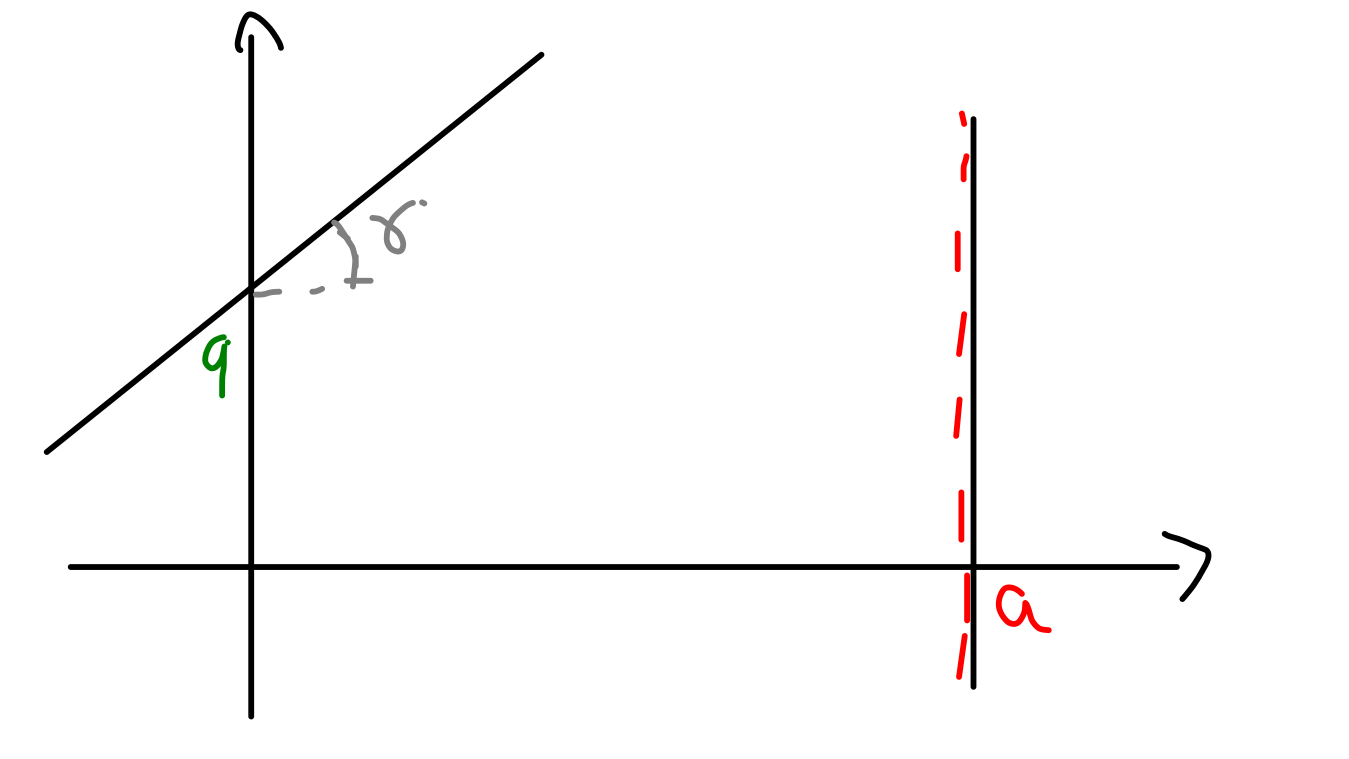
\includegraphics[width=\linewidth]{grafico_derivata_retta.png}
  	\caption{}
        \label{fig:grafico_derivata_retta.png}
\end{figure}
Dati due punti $ P_0(x_0, y_0) $ e $ P_1(x_1, y_1)$ tali che $ P_0 \not = P_1 $, qual'è la retta che passa per $ P_0 $ e $ P_1 $. \par
Impongo il passaggio $ r = \{y = mx + q\} $ allora $ P\in r \Leftrightarrow (x_0, y_0) \in \{y = mx + q\} \Leftarrow x_0,y_0$ verificata l'equazione $ y = mx + q $:

\begin{align*}
 y = mx + q \rightarrow
\begin{cases}
        P_0 \in r \\
        P_1 \in r
\end{cases}
\rightarrow
\begin{cases}
        y_0 = mx_0 + q\\
        y_1 = mx_1 + q
\end{cases}
 \rightarrow 
\begin{cases}
        y_0 = mx_0 + q\\
        y_1 - y_0 = m(x_1 - x_0) + q \rightarrow m = \frac{y_1-y_0}{x_1-x_0} * x_0\\
\end{cases}
\\
\rightarrow 
\begin{cases}
        y_0 = \\
        m = \frac{y_1-y_0}{x_1-x_0} * x_0
\end{cases}
\end{align*}
\todo{LEZ 8/4: Aggiungere lezione 10:3}
\end{document}
